\documentclass{article}
\usepackage[utf8]{inputenc}
\usepackage{subcaption}
\usepackage{amsmath}
\usepackage{amssymb}
\usepackage{hyperref}
\usepackage{titlesec}
\usepackage{xcolor}
\usepackage{fancyhdr}
\usepackage{graphicx}
\usepackage{multirow}
\usepackage[rightcaption]{sidecap}
\usepackage{verbatim}
\usepackage[backend=bibtex]{biblatex}
\graphicspath{ {./images/} }
\usepackage[ a4paper, hmargin =1.2 in, bottom =1.5 in ] { geometry }
\hypersetup{
    colorlinks=true,
    linkcolor=blue,
    filecolor=magenta,      
    urlcolor=cyan,
}

\bibliography{references}
% Add header and footer code here
% You may also add path to the images optionally


\begin{document}

% preamble
\begin{center}
    \huge
    Transformation of R.V\\ and\\ Multivariable Gaussian\\
    \large
    \vspace{5mm} %5mm vertical space
    Siddhant Mulkikar
\end{center}

% below line auto generates the table of contents
% thank me for your free 1 mark
\tableofcontents
\clearpage
\pagestyle{fancy}
\fancyhead[L]{Transformation of R.V. and Multivariate Gaussian}
\fancyhead[R]{Siddhant Mulkikar}
\fancyfoot[C]{Page \thepage}
%code of section 1, with lists
\section{Introduction}
In this article, we will study about the following topics of statistics:
\begin{itemize}
    \item Transformation of Random Variables
    \item Multivariable Gaussian
\end{itemize}
%code of section 2, make appr
\section{Transformation of Random Variables}
Given any continuous r.v. $X$ with PDF $P_{X}(x)$ and given any function g($X$)(defined on range of
$X$) we intend to find PDF associated with the r.v. $Y$ = $g(X)$.\\
For simplicity, let’s assume $g(.)$ is monotonic increasing.\\
Then by probability mass conservation,
\begin{equation*}
    P (a < X < b) = P (g(a) < Y < g(b)) =  \int_{g(a)}^{g(b)} Q^y \,dy
\end{equation*}
Using $y = g(x)$, we get the below relation upon simplification
\begin{equation*}
    Q(y) = P(g^{-1}(y))\frac{d(g^{-1}(y))}{dy}\
\end{equation*}
To handle monotonically decreasing $g(.)$ as well\footnotemark,
\footnotetext{we could have used modulus operator but I wanted things to look more complicated}
\begin{equation}
    Q(y) = \begin{cases}
        +P(g^{-1}(y))\frac{d(g^{-1}(y))}{dy}\\
        -P(g^{-1}(y))\frac{d(g^{-1}(y))}{dy}
    \end{cases}
\end{equation}
\newline
\begin{figure}[h]

    \begin{subfigure}{0.5\textwidth}
    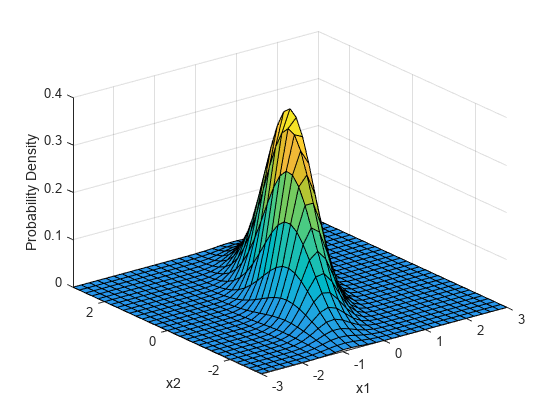
\includegraphics[width=1.0\textwidth]{multivariate_gaussian} 
    \caption{Example 1}
    \label{fig:subim1}
    \end{subfigure}
    \begin{subfigure}{0.5\textwidth}
    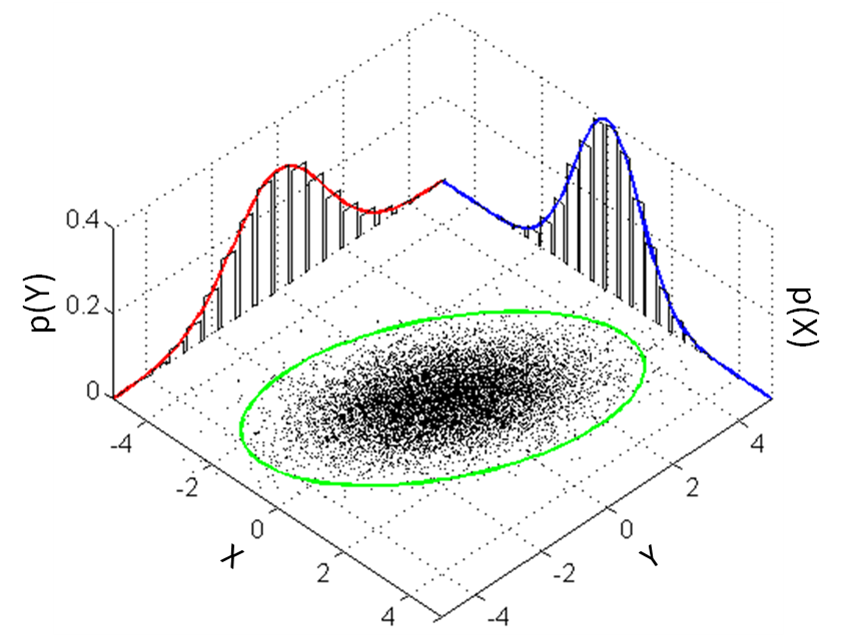
\includegraphics[width=1.0\textwidth]{multivariate_normal}
    \caption{Example 2}
    \label{fig:subim2}
    \end{subfigure}
\end{figure}
%para
% \[\]
%para.....
% \begin{equation}
% \end{equation}



% \begin{figure}[h!]
%     % code for subfigure, label them for using references
% \end{figure}

%code for section 3
\section{Multi-variate Gaussian Disribution}
\subsection{Definitions:}
Let $X$ be a vector of random variables of dimension $D$.\\
A r.v. $X$ has a joint PDF as multi-variate Gaussian distribution $\exists$ finite i.i.d. standard Gaussian
r.v. $W_{1}, W_{2},...W_{N}$ with $N>D$ such that \\
\begin{equation*}
    X = AW + \mu
\end{equation*}
Refer fig[1a] and fig[1b] for visual examples. This has many applications in machine learning, refer
[3] and [2].

\subsection{A is diagonal}
In this case, the $X_i$ are independent. The standard deviation of distribution of $X_i$ is $A_{ii}$.

\subsection{A is non-singular square matrix}
Let’s take $\mu = 0$ for simplicity.\\
Similar to univariate case, where scaling was determined by $\left|\frac{d(g^{-1}(y))}{dy}\right|$, the scaling for multi-variate
case is determined by determinant of matrix of derivatives, Jacobian matrix.\\
Also, $W = A^{-1}X$, which is a linear transformation of vector $X$. $A^{-1}$ maps a hypercube to paral-
lelepiped. If the vectors describing the hypercube are along cardinal axis, then the parallelepiped
is described by vectors which are columns of $A^{-1}$.\\
We intend to find the volume of the parallelepiped formed due to this transformation.\\
\textbf{Claim: } The volume of parallelepiped described by column vectors of matrix $A^{-1}$ is given by
$det(A^{-1})$\\
\textbf{Proof: } Addition of any scaled column of a matrix M to another column does not change the
determinant.
Therefore by Gram-Schmidt orthogonalization process the columns of $A^{-1}$ can be constructed
to be orthogonal to each other, without changing the determinant. Then multiplying by an or-
thogonal matrix would rotate the orthogonal vectors\(to align them with cardinal axis\), and this
operation would not change the determinant as well. Now the result matrix is diagonal square
matrix and the volume of the parallelepiped described by the column vectors is given by product
of diagonal elements.\\
\newline
From the above result, an infinitesimal volume $\delta$ D after transformation becomes $\delta$ D · $det(A^{-1} )$.\\
\newline
Let $C = A\cdot A^{T}$ . Then $det(A) = \sqrt{det(C)}$. The above expression can we written as\\
\begin{equation}
    P(X) = \frac{1}{(2\pi)^{D/2}}\ \cdot \frac{1}{\sqrt{det(C)}}\ \cdot exp(0.5 \cdot X^{T} \cdot C^{-1} \cdot X)
\end{equation}
% \begin{ 
%
\begin{tabular}
    {|p{3cm}|p{3cm}||p{3cm}|}
    \hline
    \multicolumn{3}{|c|}{sample sid}\\
    \hline
% % ... fill up table
\end{tabular}


% print the bibliography

\end{document}
